\documentclass[nobib]{tufte-handout}
% \documentclass[fleqn,reqno,12pt]{article}

%========================================
% Packages
%========================================

\usepackage[nographicx, nohyperref, nosubcaption, nogb4e]{mfpackages}
\usepackage{subcaption}
\usepackage{mfenvironments}
\usepackage{mfcommands}
% for info boxes
\usepackage{newfloat, caption}
\DeclareCaptionType{InfoBox}
% for table spacing
\usepackage{array, booktabs}
\usepackage{tabularray}

\usepackage{float}
\usepackage{amsmath}
\usepackage{amssymb}
\usepackage{changepage}



%========================================
% Section numbering (in the left margin)
%========================================

\setcounter{secnumdepth}{5}
\renewcommand\thesection{\arabic{section}}

% this length controls tha hanging indent for titles
% change the value according to your needs
\newlength\titleindent
\setlength\titleindent{0.7cm}

% \pretocmd{\paragraph}{\stepcounter{subsection}}{}{}
% \pretocmd{\subparagraph}{\stepcounter{subsubsection}}{}{}

\titleformat{\chapter}[block]
  {\normalfont\huge\bfseries}{}{0pt}{\hspace*{-\titleindent}}

\titleformat{\section}
  {\normalfont\Large\itshape}{\llap{\parbox{\titleindent}{\thesection\hfill}}}{0em}{}

\titleformat{\subsection}
  {\normalfont\itshape}{\llap{\parbox{\titleindent}{\thesubsection\hfill}}}{0em}{}

\titleformat{\subsubsection}
  {\normalfont\normalsize\itshape}{\llap{\parbox{\titleindent}{\thesubsubsection}}}{0em}{}

\titleformat{\paragraph}[runin]
  {\normalfont\normalsize\itshape}{}{-0.7cm}{}[\xspace \ \ \ \ ]

\titleformat{\subparagraph}[runin]
  {\normalfont\normalsize}{\llap{\parbox{\titleindent}{\thesubsubsection\hfill}}}{0em}{}

\titlespacing*{\chapter}{0pt}{0pt}{20pt}
\titlespacing*{\subsubsection}{0pt}{3.25ex plus 1ex minus .2ex}{1.5ex plus .2ex}
\titlespacing*{\paragraph}{0pt}{3.25ex plus 1ex minus .2ex}{0em}
\titlespacing*{\subparagraph}{0pt}{3.25ex plus 1ex minus .2ex}{0em}



%========================================
% Bibliography
%========================================

\bibliography{references.bib}

%========================================
% General Layout Tweaks
%========================================

% \usepackage[margin=2cm]{geometry}

% Itemize
\renewcommand{\labelitemi}{\large{$\mathbf{\cdot}$}}    % itemize symbols
\renewcommand{\labelitemii}{\large{$\mathbf{\cdot}$}}
\renewcommand{\labelitemiii}{\large{$\mathbf{\cdot}$}}
\renewcommand{\labelitemiv}{\large{$\mathbf{\cdot}$}}
% Description
\renewcommand{\descriptionlabel}[1]{\hspace\labelsep\textsc{#1}}

% Figure Captions
\usepackage{caption} % use corresponding myfiguresize!
\setlength{\captionmargin}{20pt}
\renewcommand{\captionfont}{\small}
\setlength{\belowcaptionskip}{7pt} % standard is 0pt

%========================================
% Define colors and comment functions
%========================================

\usepackage{xcolor}
\definecolor{firebrick}{RGB}{178,34,34}
\definecolor{DarkGreen}{RGB}{34,178,34} 
\definecolor{DarkOrange}{RGB}{255,100,50}
\definecolor{BackgroundR}{RGB}{235,250,250}
\renewcommand{\mf}[1]{\textcolor{firebrick}{[mf: #1]}}  
\newcommand{\lh}[1]{\textcolor{DarkOrange}{[lh: #1]}}  
% comment function for the goal of each paragraph
\newcommand{\goal}[1]{\textcolor{DarkGreen}{[goal: #1]}}
\definecolor{mathcolor}{HTML}{3C902B}
%========================================
% Configuring the R code presentation
%========================================

\usepackage{courier}
\usepackage{listings}
\usepackage{color}
% the following defines the layout for the R code
\lstset{ %
  language=R,                     % the language of the code
  basicstyle=\footnotesize\ttfamily, % size and type of the fonts that are used for the code
  numbers=left,                   % where to put the line-numbers
  numberstyle=\tiny\color{gray},  % the style that is used for the line-numbers
  stepnumber=0,                   % the step between two line-numbers. If it's 1, each line
                                  % will be numbered
  numbersep=5pt,                  % how far the line-numbers are from the code
  backgroundcolor=\color{BackgroundR},  % choose the background color. You must add \usepackage{color}
  showspaces=false,               % show spaces adding particular underscores
  showstringspaces=false,         % underline spaces within strings
  showtabs=false,                 % show tabs within strings adding particular underscores
  frame=single,                   % adds a frame around the code
  rulecolor=\color{white},        % if not set, the frame-color may be changed on line-breaks within not-black text (e.g., commens (green here))
  tabsize=2,                      % sets default tabsize to 2 spaces
  captionpos=b,                   % sets the caption-position to bottom
  breaklines=true,                % sets automatic line breaking
  breakatwhitespace=false,        % sets if automatic breaks should only happen at whitespace
  title=\lstname,                 % show the filename of files included with \lstinputlisting;
                                  % also try caption instead of title
  keywordstyle=\color{black},      % keyword style
  alsoletter={_},                  % this treats _ as a letter
  commentstyle=\color{DarkGreen}, % comment style
  stringstyle=\color{DarkOrange}, % string literal style
  escapeinside={\%*}{*)},         % if you want to add a comment within your code
  morekeywords={*, ...},           % if you want to add more keywords to the set
  deletekeywords={_}         % remove keywords from list
}

% this is for showing the R output
\lstnewenvironment{rc}[1][]{\lstset{language=R, stepnumber=1}}{}

% this is for inline R code
\newcommand{\ri}[1]{\mbox{\lstinline{#1}}\xspace}  %% Short for 'R inline'


% commands for uniform style
\newcommand{\docalc}{\emph{do}-calculus\xspace}
\newcommand{\doop}{\emph{do}-operation\xspace}
\newcommand{\mathdo}{\mathit{do}}
\newcommand{\Palt}{\ensuremath{{\color{mathcolor}{P^*}}}} % alt. Prob after "do(X)"



%========================================
% Article Header 
%========================================


\title{Causal analyses with Bayesian regression modeling: A tutorial}
\author{Lena Holzwarth \& Michael Franke}
\date{}

%========================================
% Article Body
%========================================

\begin{document}

\maketitle

\begin{abstract}
\noindent 
This tutorial provides a conceptual introduction to causal inference with the \docalc, as introduced in the work of Judea Pearl.
Unlike Pearl's original work, the tutorial showcases the use of Bayesian regression modeling to obtain causal effect estimates with quantified uncertainty.
A hands-on programming example in R is given for an artificial data set instantiating \emph{Simpson's paradox}.
\end{abstract}

\section{Motivation \& intended audience}

This tutorial has two goals: First, to introduce the reader to the concepts behind causal analysis with the \docalc \citep{pearl2000models}, and second, to perform Bayesian regression modeling to obtain not only the estimated causal effects, but also uncertainty estimates of these effects. 

Different types of readers might profit from this tutorial.
If you are new to causal inference with the \docalc, the conceptual part of this tutorial provides a basic introduction to the intuitions at the core of the \docalc, while the practical part offers a simple programming example in R to illustrate the application to a toy research question \citep{R}. 
If you are already familiar with the concepts behind the \docalc, you might want to skip to the practical application directly. 
The tutorial will assume basic familiarity with R and regression modeling. 
\marginnote{\fullcite{FrankeRoettger2019:Bayesian-regres}}
For the implementation of Bayesian regression modeling, we will use the \texttt{brms} package \citep{brms}. 
If you're unfamiliar with Bayesian regression modeling, check out, e.g., \href{https://doi.org/10.31234/osf.io/cdxv3}{{\textcolor{Red}{this tutorial $\rightarrow$}}}.

\section{Searching for Causality}

CORRELATION DOES NOT IMPLY CAUSATION! 
In scientific education, this is often one of the first lessons in statistics. 
We are told, time and again, that we should be weary of interpreting data collected by observation. 
If we want to establish a causal relationship, we are taught that there is one gold standard: the randomized experiment.
However, there are severe limitations to the randomized experiment framework. 
For some research, randomized experiments are too expensive, too unethical, or downright impossible. 
Maybe we have old data and don't know how it was obtained. 
Even if we are able to perform a randomized experiment, the independent variables we investigate might not be independent from each other.
What are we to do in these cases?

There are multiple methods to estimate causal effects from any given data set, irrespective of whether it was obtained by experimental manipulation or not. 
In this tutorial, we will introduce you to one of them: the \docalc. 
The process of causal effect estimation using the \docalc is illustrated in this flowchart:

\begin{center}
        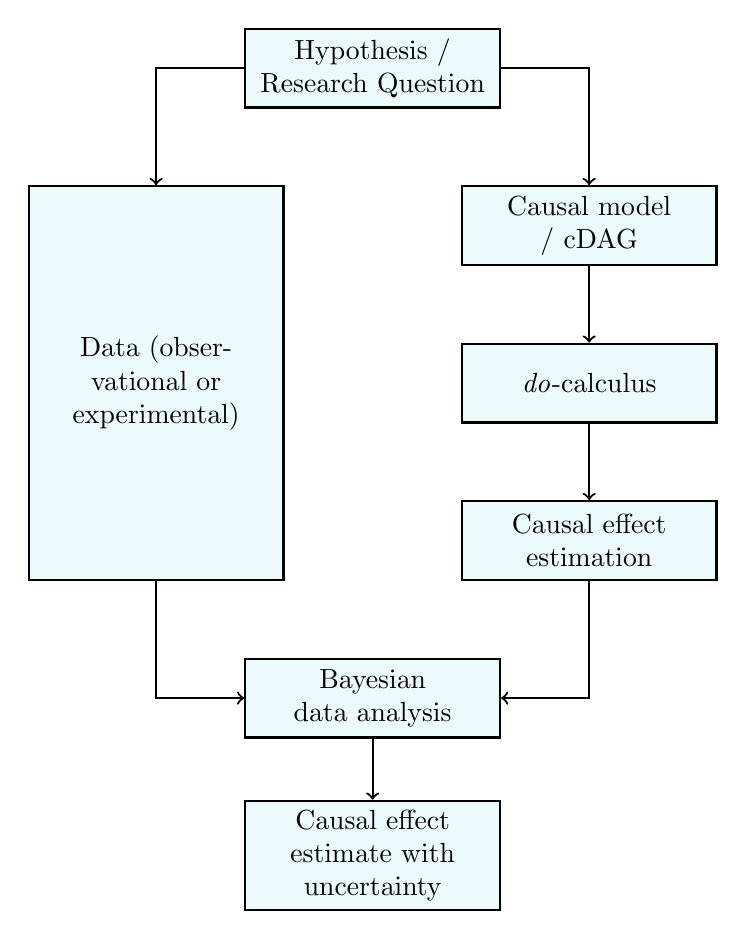
\begin{tikzpicture}[
        node distance=2cm,
        double distance=2pt,
        minimum width=3cm,
        minimum height=1cm,
        text centered, 
        text width=3cm,
        rectangle,
        thick]

    
        % NODES
        % anchors
        \node[] (ANCHOR) {};

        % hypothesis 
        \node[draw=black, fill=BackgroundR, above of = ANCHOR, node distance = 4cm] (hypothesis) {Hypothesis / Research Question};

        % data
        \node[draw=black, fill=BackgroundR, minimum height=5cm, left of = ANCHOR, node distance = 2.75cm] (data) {Data (observational or experimental)};

        % causal inference 
        \node[draw=black, fill=BackgroundR, right of = ANCHOR, node distance = 2.75cm] (do-c) {\docalc};
        \node[draw=black, fill=BackgroundR, above of = do-c] (cdag) {Causal model / cDAG};
        \node[draw=black, fill=BackgroundR, below of = do-c] (ce) {Causal effect estimation};

        % Bayesian data analysis
        \node[draw=black, fill=BackgroundR, below of = ANCHOR, node distance = 4cm] (bda) {Bayesian data analysis};
        \node[draw=black, fill=BackgroundR, below of = bda] (result) {Causal effect estimate with uncertainty};
    
        % ARROWS
        \draw[->] (hypothesis)-|(data);
        \draw[->] (data)|-(bda);
        \draw[->] (hypothesis)-|(cdag);
        \draw[->] (cdag)--(do-c);
        \draw[->] (do-c)--(ce);
        \draw[->] (ce)|-(bda);
        \draw[->] (bda)--(result);
        
        \end{tikzpicture}
    \end{center}



The tutorial is structured as follows.
Section~3 introduces a fictitious data set that will serve as our running example for this tutorial.
The data set instantiates a case of \textit{Simpson's paradox}.
In Section~4, the theoretical background to the \docalc is explained and we use a maximum-likelihood approach to estimate the causal effect in our hypothetical experiment.
Finally, Section~5 guides you through the practical application of the \docalc in a Bayesian regression modeling framework. 

\begin{InfoBox}
\centering
\colorbox{mygray}{
  \centering
  \begin{minipage}{1\textwidth}
    \medskip
    
    \emph{The Neyman-Rubin Causal Model / potential outcome framework}
    \medskip
    
    The Neyman-Rubin causal model is based on the framework of potential outcomes that a treatment would have on an individual. 
    As an example, let's consider going to college as the treatment, and future income as the outcome of interest. 
    The causal effect of going to college on the individual's future income is defined as the difference between the income with and without a college degree. 
    This notion of causal effect is a hypothetical measure, as the potential outcomes are counterfactual and only one of them can be observed.
    Importantly, the potential outcomes are treated as fixed quantities and not RVs.
    This is different from \docalc, where the outcomes are also stochastic, and the assignment of treatment is fixed/deterministic.
    The only stochastic process in the Neyman-Rubin causal model is the assignment of treatment, which depends on the observable characteristics $X$.
    These could, for example, be high school grades, socio-economic background or gender.
    Because the potential outcomes are fixed, any two individuals who share the same set of characteristics $X$ have the same potential outcomes. 
    This can be leveraged to compute the causal effect.
    For each combination of values $X$ can take, the income of individuals who went to college can be compared with that of those who didn't. 
    This procedure is called matching. 
    Because it is in most cases not easy to find individuals with exactly matching values of $X$, especially for continuous variables, there are different proposed matching methods \citep{sekhon2008neyman}.
   
    \medskip

    \emph{Structural Equation Modeling}
    \medskip

    A structural equation model (SEM) is a causal model that combines observable and latent variables.
    The causal connections between variables are represented with equations and treated as a-priori.
    SEMs can also be represented graphically in path diagrams.
    A path diagram is not the same as a cDAG, because it is not acyclic and can involve feedback relations. However, in this case, the model is underidentified and non-testable.
    The goal of a SEM is to estimate the values of latent variables from the measured values of the observable variables. 
    SEMs can be evaluated with measures of model fit. 
    In case of a bad fit, the causal assumptions underlying model formulation can be regarded as falsified \citep{bollen2013eight}. 

    It has been shown that the potential outcome framework and structural equation modeling are logically equivalent \citep{galles1998axiomatic, halpern2000axiomatizing}. 
    \citet{pearl2000models} combined features of the potential outcome framework and SEM to formulate the structural causal model as a general theory of causation.
    
    \medskip
    
    
  \end{minipage} 
}
\begin{center}
Info Box 1: Alternatives to the \docalc for causal inference.
\end{center}
\end{InfoBox}    

\newpage

\section{Fictitious data \& Simpson's paradox}\label{sec:experiment}

To guide you through the steps of estimating causal effects with the \docalc, we'll look at an example.
Let's assume that we work in a hospital and want to test the effect of a new drug. 
Because this drug is still in an experimental phase, we can't randomly assign it to patients. 
Instead, we ask them if they would be willing to test the drug.
In our experiment, we have a random variable (RV) \textsc{drug intake} with two possible values: \textsc{take} for the participants consenting to test the drug and \textsc{refuse} for those who declined. 
The patients are also sorted into two groups. 

\begin{table}
\centering
\caption{Recovery rates after refusing or taking the drug}
\label{tab:anonymous}
\begin{tblr}{crcrc}
    \hline
    & \SetCell[c=2]{c} \textsc{refuse}&&\SetCell[c=2]{c}\textsc{take}\\
    \hline
    \textsc{group 1}& $\frac{234}{270}$ & (\textcolor{DarkOrange}{87\%}) & $\frac{81}{87}$ & (\textcolor{DarkGreen}{93\%})\\
    \textsc{group 2}& $\frac{55}{80}$ & (\textcolor{DarkOrange}{68\%}) & $\frac{192}{263}$ & (\textcolor{DarkGreen}{73\%})\\
    $\Sigma$& $\frac{289}{350}$ & (\textcolor{DarkGreen}{83\%}) & $\frac{273}{350}$ & (\textcolor{DarkOrange}{78\%})\\
    \hline
\end{tblr}
\end{table}   

\marginnote{The distribution of recovery rates is taken from a real-life medical study \citep{charig1986comparison} and was first discussed in relation to Simpson's Paradox by \citet{julious1994confounding}. The hypothetical experimental setup and the labels of the RVs come from \citet{pearl2000models}.}
In Table \ref{tab:anonymous}, we can see the results of our study. 
We see that overall, 83\% of patients who refused the drug recovered from their disease, while only 78\% of the drug-takers did. 
This does not bode well for our drug.
However, when we look at each group in isolation, we see that within each group, the drug-takers had a slightly higher recovery rate.
This phenomenon is an instance of \textit{Simpson's Paradox}: Splitting the participants into sub-groups yields different results compared to analyzing all data at once.
This makes the interpretation of our results very difficult: should we use the group-wise results and conclude that the drug is helpful, or should we use the overall results which indicate that the drug is harmful? 
Without further information, specifically on how the groups were formed, we can't take this decision.
This illustrates an important point for statistical analysis: the data alone is not enough to reach conclusions.
The data can't speak for itself. 
We need to be data-literate, so to speak, and bring our knowledge about where the data comes from to bear.

Let's see how adding information about the groups helps our effort to interpret the results. 
We consider two scenarios.
In the first scenario, the participants were grouped by gender (which is treated as a binary variable for the purposes of this example).
\textsc{gender} could be relevant because the drug might have different effects on the male and female body. 
However, \textsc{gender} might also influence the decision to take the drug, e.g., by one gender being more risk averse than the other. 
With the updated group names, the results are displayed in Table \ref{tab:combined}.
How should we interpret these results?\footnote{The correct answer would, of course, be `not at all' - We haven't done our causal analysis yet, this pattern is merely a correlation.}
Our intuition might be that the drug is in fact beneficial, because for men and women, the chances of recovery are higher for those who took the drug.

\begin{table*}[t]

\bigskip

\hline
    
    \centering
    
    \begin{subtable}{0.48\textwidth}
\centering
\caption{Recovery rates for different genders}
\label{tab:gender}
\begin{tblr}{crcrc}
    \hline
    & \SetCell[]{c} \textsc{refuse}&&\SetCell[c=2]{c}\textsc{take}\\
    \hline
    \textsc{men}& $\frac{234}{270}$ & (\textcolor{DarkOrange}{87\%}) & $\frac{81}{87}$ & (\textcolor{DarkGreen}{93\%})\\
    \textsc{women}& $\frac{55}{80}$ & (\textcolor{DarkOrange}{68\%}) & $\frac{192}{263}$ & (\textcolor{DarkGreen}{73\%})\\
    $\Sigma$& $\frac{289}{350}$ & (\textcolor{DarkGreen}{83\%}) & $\frac{273}{350}$ & (\textcolor{DarkOrange}{78\%})\\
    \hline
\end{tblr}
    \end{subtable}
    %
    \begin{subtable}{0.48\textwidth}

\centering
\caption{Recovery rates for different values of blood pressure}
\label{tab:bp}
\begin{tblr}{crcrc}
    \hline
    & \SetCell[c=2]{c} \textsc{refuse}&&\SetCell[c=2]{c}\textsc{take}\\
    \hline
    \textsc{low}& $\frac{234}{270}$ & (\textcolor{DarkOrange}{87\%}) & $\frac{81}{87}$ & (\textcolor{DarkGreen}{93\%})\\
    \textsc{high}& $\frac{55}{80}$ & (\textcolor{DarkOrange}{68\%}) & $\frac{192}{263}$ & (\textcolor{DarkGreen}{73\%})\\
    $\Sigma$& $\frac{289}{350}$ & (\textcolor{DarkGreen}{83\%}) & $\frac{273}{350}$ & (\textcolor{DarkOrange}{78\%})\\
    \hline
\end{tblr}
\end{subtable}

\bigskip

\hline

\bigskip

    
    \label{tab:combined}
    \caption{Changing the group names changes our intuitions about the causal effect}
    
\end{table*}

Table \ref{tab:combined} also shows a second version of the same experiment. 
Here, the participants were not grouped by gender, but by their blood pressure as measured \textit{after} taking the drug.
Participants are divided into groups with high or low blood pressure. 
In this case, our intuition is likely different. 
Because blood pressure is measured after drug administration and is likely to be influenced by the drug, it seems that the groupings into \textsc{high} and \textsc{low} are not as informative, and we should instead focus on the overall results, that tell us that the drug might even be harmful.

Why is it that we interpret the data differently, depending on the group labels? 
The reason is that the different labels tell us something about the causal structure of our experiment.
To bring our intuitions about causal dependencies to the fore, the following section looks at 
how to determine the causal structure in a data-generating process (\textit{\nameref{sec:step1}}), 
and how to use this information to estimate causal effects (\textit{\nameref{sec:step2}}).

\begin{InfoBox}
\centering
 \colorbox{mygray}{
    \begin{minipage}{1\textwidth}
    \medskip
    \emph{Directed acyclic graphs (DAGs) for causal analysis}
    \medskip

    DAGs can be used to illustrate the causal relationships between events or RVs. 
    %For simplicity, we only consider binary RVs.
    When two nodes in a causal DAG (cDAG) are connected, the RVs that they represent are statistically dependent.
    The RV with the outgoing edge causally influences the RV with the incoming edge.
    cDAGs must be directed and acyclic because causal relationships are one-way only. 
    \begin{center}
        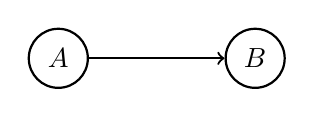
\begin{tikzpicture}[
        node distance = 1.25cm,
        double distance = 2pt,
        minimum size=0.75cm,
        circle,
        thick]
    
        % NODES
        % anchor
        \node[] (anchor) {};
        % node X
        \node[draw=black, left of = anchor] (A) {$A$};
        % node Y
        \node[draw=black, right of = anchor] (B) {$B$};
    
        % ARROWS
        \draw[->] (A)--(B);
        \end{tikzpicture}
    \end{center}
    In this example, the RV $A$ influences the value of the RV $B$. 
    Importantly, this relationship is not necessarily  deterministic, s.t. $A=1$ always implies $B=1$. 
    Instead, it is usually stochastic, s.t. some value of $A$ makes it more likely for $B$ to take a certain value, e.g., $P(B=1 \mid A=1) > P(B=0 \mid A=1)$.

    cDAGs can be comprised of infinitely many nodes.
    All of their relationships can be brought down to a limited set of shapes.
    Some of these are shown below: the chain and the fork.
    Understanding these granular causal structures helps to interpret more complex cDAGs.
    
    \begin{center}
        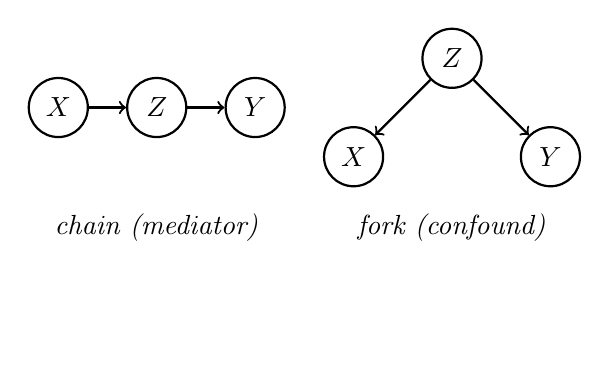
\begin{tikzpicture}[
        node distance = 1.25cm,
        double distance = 2pt,
        minimum size=0.75cm,
        circle,
        thick]
    
        % NODES
        % anchors
        \node[] (ANCHOR) {};
        
        \node[draw=black, left of = ANCHOR, node distance = 3.75cm] (anchor_chain) {$Z$};
        \node[below of = ANCHOR, node distance = 0.625cm] (anchor_fork) {};
        
        % chain
        \node[draw=black, left of = anchor_chain] (chainX) {$X$};
        \node[draw=black, right of = anchor_chain] (chainY) {$Y$};
        \node[below of = anchor_chain, node distance = 1.525cm] (chain_cap) {\textit{chain (mediator)}};
        
        % fork
        \node[draw=black, left of = anchor_fork] (forkX) {$X$};
        \node[draw=black, right of = anchor_fork] (forkY) {$Y$};
        \node[draw=black, above of = anchor_fork] (forkZ) {$Z$};
        \node[below of = anchor_fork, node distance = 0.9cm] (fork_cap) {\textit{fork (confound)}};

    
        % ARROWS
        \draw[->] (chainX)--(anchor_chain);
        \draw[->] (anchor_chain)--(chainY);
        \draw[->] (forkZ)--(forkX);
        \draw[->] (forkZ)--(forkY);
        \end{tikzpicture}
    \end{center}
    
    \vspace{-1.25cm}
    In a chain, $X$ and $Y$ are causally dependent: $X$ influences the value of the mediator $Z$, which influences $Y$. 
    Using the example of our hypothetical experiment, $X$ could be a drug which influences the blood pressure level $Z$, which influences the likelihood of recovery $Y$.
    However, $X$ and $Y$ are independent conditioned on $Z$.
    If the value of blood pressure $Z$ is known, the value of $X$ (drug or no drug) gives us no further information about the recovery $Y$, because the only way in which the drug influences recovery is through adjusting the level of blood pressure.

    In a fork, $Z$ acts as a confound on $X$ and $Y$. 
    $X$ and $Y$ are dependent, because they have a common cause in $Z$. 
    $Z$ could be a variable for exercise, which influences both weight $X$ and danger of a heart disease $Y$.
    $X$ and $Y$ become independent conditioned on $Z$. 
    This is because when the amount of exercise $Z$ is given, knowing the value of a person's weight $X$ yields no further information on their risk of cardiac disease $Y$.

    For a visual explanation of these causal structures see  \href{https://youtu.be/mBEA7PKDmiY?si=Ihio7ZXJSuct4J30}{{\color{Red}{this lecture}}} by Richard McElreath.
    \medskip
  \end{minipage} 
}
\begin{center}
Info Box 2: Background on visually displaying causal relationships.
\end{center}
\end{InfoBox}


\section{Causal inference with the \docalc} \label{sec:theory}
\subsection{Step 1: Establish the Causal Structure} \label{sec:step1}


Why do we interpret the data from our two experiments differently, even though the numbers are exactly the same?
It is because the data is not the only information we have: We also know how this data was obtained and how the variables are most likely related. 
These observations, although not present in the data, still inform our intuitive judgement of the situation.
We know that \textsc{gender} ($G$) might have an influence on the decision of \textsc{drug intake} ($D$), while the taking of the drug doesn't change ones gender.
In the case of \textsc{blood pressure} ($B$), we know that it was measured after taking or refusing the drug. 
\marginnote{
    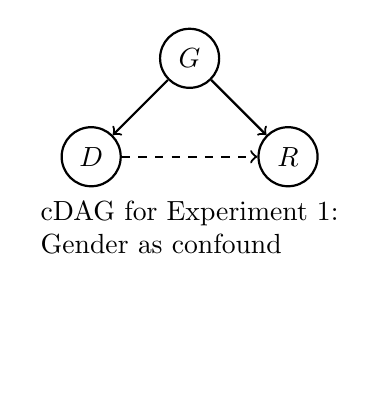
\begin{tikzpicture}[
        node distance = 1.25cm,
        double distance = 2pt,
        minimum size=0.75cm,
        circle,
        thick]
        % NODES
        % anchor
        \node[] (anchor) {};
        % node X
        \node[draw=black, left of = anchor] (D) {$D$};
        % node Y
        \node[draw=black, right of = anchor] (R) {$R$};
        % node Z
        \node[draw=black, above of = anchor] (G) {$G$};
        % caption node
        \node[below of = anchor, align = left, node distance = 0.9cm] (Cap) {cDAG for Experiment 1: \\Gender as confound}; 
        
        % ARROWS
        \draw[->] (G)--(D);
        \draw[->] (G)--(R);
        \draw[->, dashed] (D)--(R);
    \end{tikzpicture}
}
\marginnote{
    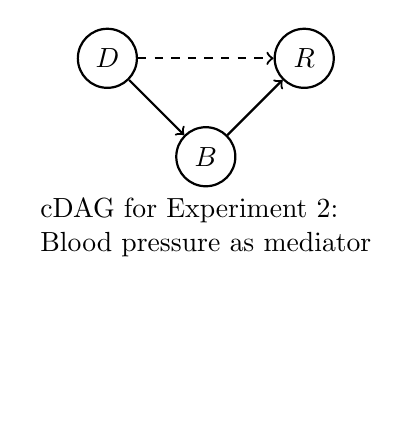
\begin{tikzpicture}[
        node distance = 1.25cm,
        double distance = 2pt,
        minimum size=0.75cm,
        circle,
        thick]
        % NODES
        % anchor
        \node[] (anchor) {};
        % node X
        \node[draw=black, left of = anchor] (D) {$D$};
        % node Y
        \node[draw=black, right of = anchor] (R) {$R$};
        % node Z
        \node[draw=black, below of = anchor] (B) {$B$};
        % caption node
        \node[below of = B, align = left, node distance = 0.9cm] (Cap) {cDAG for Experiment 2: \\Blood pressure as mediator}; 
        
        % ARROWS
        \draw[->] (D)--(B);
        \draw[->] (B)--(R);
        \draw[->, dashed] (D)--(R);
    \end{tikzpicture}
}
It therefore shouldn't have influenced the decision to take the drug. 
However, it is possible that the drug has an influence on blood pressure.
In both cases, we hypothesize that the drug has a positive effect on the patients' \textsc{recovery} ($R$).
Before starting with our analysis, we should make these causal relationships explicit.

One way to make intuitions about causal dependency explicit, is to illustrate them in a so-called \textit{causal directed acyclic graph} (cDAG).
The nodes in a cDAG represent events, measurements or random variables relevant for our data analysis.
We draw a directed arrow from one node to another if we think that, simply speaking, the former may have a causal effect on the latter. 
The precise details of cDAGs, their relation to causality and stochastic (in-)dependence, are important for advanced applications of causal inference with the \docalc.
As the motivation for this tutorial is to provide a first conceptual feeling of what can be done in this framework, Info Box~2 covers only some of the basics in a non-mathematical survey.

In the cDAGs for our experiments, which are drawn on the right side on this page, the causal connection between \textsc{drug intake} and \textsc{recovery} is drawn with a dashed arrow.
This indicates that the causal relationship between $D$ and $R$ is not yet established, but currently the subject of investigation.
All other connections in the graph are treated as factual.
\marginnote{The idea of prior knowledge influencing the analysis is familiar to Bayesians. 
However, there is one difference: in Bayesian statistics, the influence of the prior decreases with the increase of data.
The \textit{a-priori} causal assumption always influence the outcome.}
They are considered \textit{a-priori} assumptions. 
Of course, this approach bears some risks.
If we assume the wrong causal relationships, our resulting analysis will also yield wrong results.
However, it is important to note that this is the case for all statistical inference methods.
Any decision on including or excluding a certain variable from statistical analysis is implicitly an assumption about the causal structure connecting the RVs.
Formulating a specific cDAG can thus improve accountability by making the underlying assumptions explicit and easily understandable.

\marginnote{\emph{"All causal inferences based on statistical models are implicitly based on a causal structure"} \citep{shrier2008reducing}}
The construction of a cDAG and the question of which variables to include are challenging tasks, especially because in many application cases, the causal structures under observation will be much more complicated than the limited ones given here.
In many cases, it might be impossible to decide between two possible cDAGs.
In these instances, \citet{shrier2008reducing} suggest to perform the analyses on all plausible versions of the DAG.
If the different versions yield different results, all results should be presented. 
In their words: 
\marginnote{From a Bayesian point of view, we can also assign a prior probability to all candidate cDAGs and present, in addition to the estimates of causal effects for each case, a prior-weighted average, similar to other cases of model averaging in Bayesian analysis.}
\begin{quote}
\emph{
Not using the causal approach because of uncertainty on which is the correct DAG simply means that one is allowing chance rather than rational deliberation to make the choice among the different causal diagrams.    
}
\end{quote}

Once we have settled on one (or several) cDAGs, the base for our causal analysis is set, and we can continue with the second step: the intervention.


\subsection{Step 2: Intervene} \label{sec:step2}

The key to inferring causation is intervention.
This is what constitutes the power of the controlled randomized trial setup (if done well) in experimental research.
But what if we cannot, for whatever reason, interfere in the data-generating process?
Is it possible to simulate an intervention for data that is already generated?

\marginnote{"When we merely observe the value that a variable takes, we are learning about the value of the variable when it is caused in the normal way, as represented in our causal model. 
Information about the value of the variable will also provide us with information about its causes, and about other effects of those causes. 
However, when we intervene, we override the normal causal structure, forcing a variable to take a value it might not have taken if the system were left alone" \citep{sep-causal-models}.}

Indeed, as Pearl has argued prominently, simulated intervention on a random variable, so to speak, is possible in some cases (but not always). 
When we simulate an intervention, we do \textit{as if} we had manipulated the relevant variable, which means that we cut off all influence from upstream causes of that variable, thus possibly creating a modified (pruned, lesioned) cDAG.
We then use the data to estimate the effect that different values of the relevant variable have in this modified cDAG.
In our running example, we want to vary the variable \textsc{drug intake} ($D$), to measure the effects this has on \textsc{recovery} ($R$).
The causal effect of taking the drug can be estimated by \textit{pretending} that the experimenters had randomly assigned either the drug, or placebos to the patients and then comparing the recovery outcomes of the two groups. 
In this fictitious scenario, $D$ is the result of random manipulation and thus has no causal ancestors.

Handling such simulated interventions is the main job description of the \docalc. 
Instead of overwriting the value of a RV by randomization, we can do it via the \doop.
In the \doop $\mathdo(D=d)$, we set $D$ to a fixed value $d \in \{0,1\}$.\footnote{The assigned value need not be binary, this is only the case in our experiment where one can either take ($D=1$) the drug or else refuse it ($D=0$).}
Because the intervention overwrites the normal causal structure, the \doop removes any causal influences on $D$.
In the graphical representation, this means that we can remove any incoming arrows on the independent RV.
In the cDAG for Experiment 1, $\mathdo(D=d)$ leads to the removal of the causal influence of $G$ on $D$. 
In Experiment 2, the \doop has no effect at all, because there were no incoming arrows on $D$ to begin with.
\marginnote{
    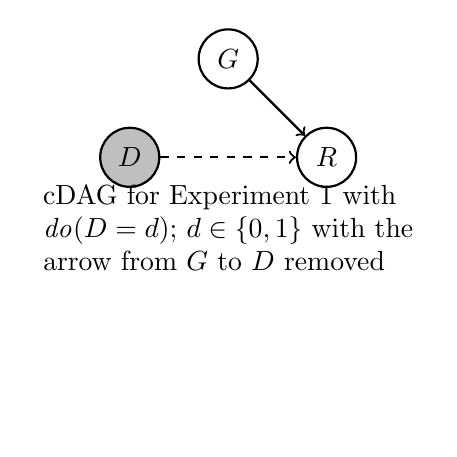
\begin{tikzpicture}[
        node distance = 1.25cm,
        double distance = 2pt,
        minimum size=0.75cm,
        circle,
        thick]
        % NODES
        % anchor
        \node[] (anchor) {};
        % node X
        \node[draw=black, fill=lightgray, left of = anchor] (D) {$D$};
        % node Y
        \node[draw=black, right of = anchor] (R) {$R$};
        % node Z
        \node[draw=black, above of = anchor] (G) {$G$};
        % caption node
        \node[below of = anchor, align = left, node distance = 0.9cm] (Cap) {cDAG for Experiment 1 with\\$\mathdo(D=d)$; $d \in \{0,1\}$ with the\\arrow from $G$ to $D$ removed}; 
        
        % ARROWS
        \draw[->] (G)--(R);
        \draw[->, dashed] (D)--(R);
    \end{tikzpicture}
}
\marginnote{
    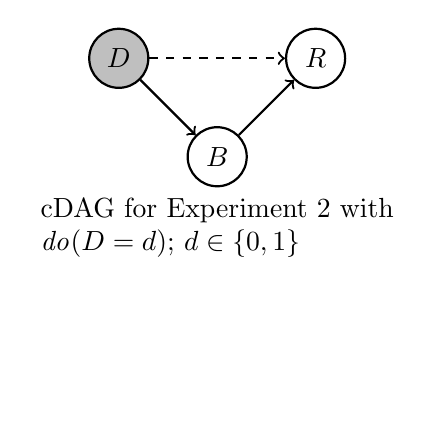
\begin{tikzpicture}[
        node distance = 1.25cm,
        double distance = 2pt,
        minimum size=0.75cm,
        circle,
        thick]
        % NODES
        % anchor
        \node[] (anchor) {};
        % node X
        \node[draw=black, fill=lightgray, left of = anchor] (D) {$D$};
        % node Y
        \node[draw=black, right of = anchor] (R) {$R$};
        % node Z
        \node[draw=black, below of = anchor] (B) {$B$};
        % caption node
        \node[below of = B, align = left, node distance = 0.9cm] (Cap) {cDAG for Experiment 2 with\\$\mathdo(D=d)$; $d \in \{0,1\}$}; 
        
        % ARROWS
        \draw[->] (D)--(B);
        \draw[->] (B)--(R);
        \draw[->, dashed] (D)--(R);
    \end{tikzpicture}
}

Let's pause here for a second and reflect on this.
We want to mimic the effects of something like an experimental intervention in a randomized control trial.
The main property that makes such experimental manipulation effective is that the relevant variable (here: $D$) was not allowed to just happen, so to speak.
Some god-like external force (the experimenters) messed up the normal causal flow, interrupted it and just set the variable to whatever they liked, no matter how likely it might have happened on its own had we not stepped in the normal courses of events. 
That is, essentially, the main property that makes experimental manipulation work.
And it is exactly this (cutting off the prior causal influences on the relevant variable ($D$)) that the \docalc implements.
In other words, the \docalc is not some crazy math-voodoo but the most straightforward implementation of what we intuitively consider to be (the power of) systematic experimental manipulation.

Okay, so we have a way of formally representing simulated interventions.
Great!
But how do we get from virtual interventions to a causal effect estimation? 
And why are we allowed to pretend that an intervention has happened, when the data we have are obtained from a completely different causal structure?
The following subsections will guide you through a mathematical example to obtain the MLE estimates of the causal effect in our two experiment scenarios and explain the mathematical intuition behind why we can (in some cases) treat the data as if it was the product of experimental manipulation.

\subsection{MLE for Experiment 1: gender as confound}

The key to understanding the \docalc is to think of a "virtual intervention" as a thought experiment: how would the causal relations be if we had actually intervened on the relevant variable?
In this imagined scenario, we would have seen data generated by a joint probability distribution $\Palt$.
Of course, the actual data we have is \textit{not} a sample from $\Palt$, but rather from a joint probability distribution $P$, which follows the dependencies of the assumed cDAG.
So, we would like to use the data, which actually comes from $P$, to estimate ---if possible--- aspects of $\Palt$.
As we said before, sometimes this cannot possibly work; but sometimes it can.
Here is an example of the latter.

Suppose we have data as in Table \ref{tab:combined}, which we assume is generated from joint probability distribution $P$.
In the cDAG that (by our working assumption) underlies $P$, variable $D$ was merely observed, not manipulated.
However, we can imagine a case where the joint probability distribution on variables follows $\Palt$ instead, where $D$ was actually experimentally manipulated, so that all upstream causal influences are suppressed.
We now introduce a new piece of notation to write $P\left(R=r \mid \mathdo(D=d)\right)$ for the conditional probability of recovery $R$ given that the drug administration $D$ had been manipulated.
In effect, the conditional probability $P\left(R=r \mid \mathdo(D=d)\right)$ with an imaginary intervention is defined as the conditional probability $\Palt \left(R = r \mid D=d \right)$ under the unobserved probabilities $\Palt$. 
You can think of the \doop as a kind of jumping board to get from the actual probability distribution $P$ to the imagined $\Palt$.
However, this "fictitious" conditional probability cannot be calculated based on $P$ without further ado, because it assumes that the data-generating process was a different one, namely one that follows the joint distribution $\Palt$.
This makes the \doop seem kind of pointless, like notation juggling or just some renaming trick.
But, the good news is that in some cases, the data obtained from process $P$ can be used to safely estimate all the relevant aspects of $\Palt$, so that we can eventually estimate the desired $P\left(R=r \mid \mathdo(D=d)\right)$ entirely from the non-interventionist data at hand. 

How does this work? 
As motivated above, by definition we have:
%
\begin{align*}
P\left(R=r \mid \mathdo(D=d)\right) 
& = \Palt \left(R = r \mid D=d \right)
\end{align*}
%
Since we are now entirely in a "do"-free case, the usual rules of probability apply:
%
\begin{align*}
\Palt \left(R = r \mid D=d \right)
& = 
\sum_{g} \Palt \left(R = r \mid D=d, G=g \right) \ \Palt \left( G=g \mid D=d \right)
\end{align*}
%
Since in $\Palt$ variable $D$ and $G$ are assumed to be independent, we can simplify:
%
\begin{align*}
& \sum_{g} \Palt \left(R = r \mid D=d, G=g \right) \ \Palt \left( G=g \mid D=d \right) \\
= & \sum_{g} \Palt \left(R = r \mid D=d, G=g \right) \ \Palt \left( G=g \right)
\end{align*}
%
And now the magic unfolds, when we realize that all of the "ingredients" in the last expression, though expressed as probabilities from $\Palt$ can be safely estimated from data generated from $P$, i.e., our actual data.
Why? --- Because we assume that the data-generating processes behind $P$ and $\Palt$ only differ with respect to the dependence of $G$ and $D$, but the remaining (conditional) probabilities, though expressed in $\Palt$, are identical in $P$. 
So, we may conclude that, in this particular case, it is possible to "calculate away" the imaginary intervention effect by expressing it entirely in quantities safely estimable from the data at hand, since:
%
\begin{align*}
& \sum_{g} \Palt \left(R = r \mid D=d, G=g \right) \ \Palt \left( G=g \right)
\\
= & 
\sum_{g} P\left(R = r \mid D=d, G=g \right) \ P\left( G=g \right)
\end{align*}
%
The full derivation is repeated more concisely here:
%
\begin{align*}
P&\left(R=r \mid \mathdo(D=d)\right) \\
&= \Palt \left(R = r \mid D=d \right)
& \color{gray}{\text{[by \ def.]}}\\
&= \sum_{g} \Palt \left(R = r \mid D=d, G=g \right) \ \Palt \left( G=g \mid D=d \right)
& \color{gray}{\text{[std. prob.]}}\\
&= \sum_{g} \Palt \left(R = r \mid D=d, G=g \right) \ \Palt \left( G=g \right)
& \color{gray}{\text{[cond. indep.]}}\\
&= \sum_{g} P\left(R = r \mid D=d, G=g \right) \ P\left( G=g \right)
& \color{gray}{\text{[same in $P$]}}
\end{align*}

Now, we can compute the drug's causal effect on recovery by plugging in the numbers from our observational study in Table \ref{tab:combined}.
We compare the recovery rates for cases where the patients took ($P(R=1\mid \do(D=\textsc{take}$) or refused the drug ($P(R=1\mid \do(D=\textsc{take}$):
\begin{equation}
\begin{split}
P(R=1\mid \mathdo(D=\textsc{take})
&= \sum_{g\in \{0,1\}} P(R=1\mid G=g; D=1) P(G=g)\\
&= \frac{81}{87} \cdot \frac{357}{700} + \frac{192}{263} \cdot \frac{343}{700} \approx 0.83
\end{split}
\end{equation}
\begin{equation}
\begin{split}
P(R=1\mid \mathdo(D=\textsc{refuse})
&= \sum_{g\in \{0,1\}} P(R=1\mid G=g; D=0) P(G=g)\\
&= \frac{234}{270} \cdot \frac{357}{700} + \frac{55}{80} \cdot \frac{343}{700} \approx 0.78
\end{split}
\end{equation}
According to these point-valued estimates, patients who take the drug approximately have a 0.83 chance of recovery, while not taking the drug yields a 0.78 chance to recover. 
To get the causal effect estimate, we simply have to compare the predicted outcome for patients taking the drug with those refusing it.
The estimated causal effect of \textsc{drug intake} on \textsc{recovery} is thus $P(R=1\mid \mathdo(D=\textsc{take})-P(R=1\mid \mathdo(D=\textsc{refuse}) \approx 0.05$, meaning that the drug increases the chance of patients to recover by 5\%.

\subsection{MLE for Experiment 2: blood pressure as mediator}

In experiment 2, the independent variable $D$ is not causally dependent on any other RV. 
The \doop, whose job it is to remove causal influences on the independent variable, thus doesn't have an effect in this case, because there aren't any causal influences on $D$ to begin with.
This means that the observed distribution $P$ is identical to the hypothetical distribution $\Palt$. 
The probability for recovery, in this case, is just $P(R=1\mid D=d)$:

\begin{align*}
P&\left(R=1\mid \mathdo(D=d)\right) \\
&= \Palt \left(R=1\mid D=d\right) 
& \color{gray}{\text{[by \ def.]}} \\
&= \sum_{b} \Palt\left(R=1\mid B=b; D=d)\right) \Palt\left(B=b\mid D=d\right)
& \color{gray}{\text{[std. prob.]}}\\
&= \sum_{b} P\left(R=1\mid B=b; D=d\right) P\left(B=b\mid D=d\right)
& \color{gray}{\text{[same in $P$]}}\\
&= P\left(R=1\mid D=d\right)
\end{align*}



We can thus directly read the maximum-likelihood estimates from the \textsc{recovery} frequencies observed in the experiment:
\begin{equation}
\begin{split}
P(R=1\mid \mathdo(D=\textsc{take})
= P(R=1\mid D=1)
= \frac{273}{350} \approx 0.78
\end{split}
\end{equation}
\begin{equation}
\begin{split}
P(R=1\mid \mathdo(D=\textsc{refuse})
= P(R=1\mid D=0)
= \frac{289}{350} \approx 0.83
\end{split}
\end{equation}

So, for this case, we estimate that the causal effect of \textsc{drug intake} on \textsc{recovery} is $P(R=1\mid \mathdo(D=\textsc{take})-P(R=1\mid \mathdo(D=\textsc{refuse}) \approx -0.05$.
According to this estimation, taking the drug might actually worsen the chances to recover.
\medskip

Note that while we are able to compute a causal effect estimate by hand using a maximum-likelihood estimation approach, we don't get a measure of certainty without further ado. 
Numerically a causal effect of about 5\% may seem pretty small, so how are we to tell whether this is reliably different from a causal effect size of zero?
This is where the Bayesian approach comes into play.
How to use Bayesian regression modeling to not only estimate causal effects, but also their certainties, is the topic of the remainder of this tutorial.

\section{Tackling Simpson's Paradox with Bayesian Regression} \label{sec:programming}

\marginnote{The entire code is available at \href{https://github.com/michael-franke/BayesReg-CausalInference}{{\texttt{https://github.com/michael-franke/\\BayesReg-CausalInference}}}.} 
Having established the conceptual basics, let's now dive into the programming part. 
First, we set up the environment and load the required packages:
\begin{minipage}[]{\textwidth}
\begin{lstlisting}[language=R]
# packages for Bayesian regression modeling
library(brms) 
# install faintr from Github (easy evaluation of brm models)
devtools::install_github("michael-franke/faintr")

# packages for data wrangling
library(tibble)     # dataframes 
library(tidyr)      # for re-grouping dataframes
library(dplyr)      # intuitive data manipulation

# option for Bayesian regression models: 
# use all available cores for parallel computing
options(mc.cores = parallel::detectCores())

# random seeding for reproducibility
set.seed(123)
\end{lstlisting}
\end{minipage}

\vspace{-0.5cm}
Then, we create a dataset with the values from Table \ref{tab:combined} and transform it into the required shape.

\begin{minipage}[]{\textwidth}
\begin{lstlisting}[language=R]
# generate dataset with Simpson's paradox
data_simpsons_paradox <- tibble(
  gender = c("Male", "Male", "Female", "Female"),
  bloodP = c("Low", "Low", "High", "High"),
  drug = c("Take", "Refuse", "Take", "Refuse"),
  k = c(81, 234, 192, 55),
  N = c(87, 270, 263, 80),
  proportion = k/N
)

# cast into long format
data_SP_long <- rbind(
  data_simpsons_paradox |> 
    uncount(k) |>
    mutate(recover = TRUE) |>
    select(-N, -proportion), 
  data_simpsons_paradox |>
    uncount(N-k) |>
    mutate(recover=FALSE) |>
    select(-k, -N, -proportion)
  )

\end{lstlisting}
\end{minipage}

\vspace{-0.5cm}
Now, we can start modeling!

\subsection{Experiment 1: Gender as confound}

In experiment 1, the effectiveness of the drug is confounded by \textsc{gender}.
As we have derived in Section \ref{sec:theory}, we can estimate the probability of recovery with or without the drug as 
$$P \left(R=r \mid \mathdo (D=d)\right) = \sum_{g} P\left(R = r \mid D=d, G=g \right) \ P\left( G=g \right)$$
To obtain the probability estimate, we perform Bayesian regression modeling.
We need to model two probability distributions: first, the distribution of \textsc{gender}, $P\left( G=g \right)$ and second, the conditional probability of \textsc{recovery}, $P\left(R = r \mid D=d, G=g \right)$.
We will explain two different sampling strategies to obtain these estimates.
\emph{Method A} is more intuitive, while \emph{Method B} is more efficient, but both are equally adequate.

\begin{center}
        \begin{tikzpicture}[
        node distance=2cm,
        double distance=2pt,
        minimum width=2cm,
        minimum height=1cm,
        text centered, 
        text width=2.5cm,
        rectangle,
        thick]

    
        % NODES
        % anchors
        \node[] (ANCHOR_A) {};
        \node[right=5cm of ANCHOR_A] (ANCHOR_B) {};

        % Method A
        \node[above of = ANCHOR_A, node distance = 3cm] (A) {\emph{Method A}};
        
        \node[draw=black, fill=BackgroundR, right of = ANCHOR_A, node distance = 1.5cm] (sampleA) {sample participants};

        \node[left of = ANCHOR_A, node distance = 1.5cm] (ANCHOR_recov_A) {};

        \node[draw=black, fill=BackgroundR, above of = sampleA] (genderA) {model \textsc{gender}};

        \node[draw=black, fill=BackgroundR, above of = ANCHOR_recov_A] (recovA) {model \textsc{recovery}};

        \node[draw=black, fill=BackgroundR, below of = ANCHOR_A] (estimateA) {estimate mean recovery of sample};

        % Method B
        \node[above of = ANCHOR_B, node distance = 3cm] (B) {\emph{Method B}};
        
        \node[draw=black, fill=BackgroundR, right of = ANCHOR_B, node distance = 1.5cm] (sampleB) {estimate mean gender};

        \node[draw=black, fill=BackgroundR, left of = ANCHOR_B, node distance = 1.5cm] (ANCHOR_recov_B) {estimate mean recovery};

        \node[draw=black, fill=BackgroundR, above of = sampleB] (genderB) {model \textsc{gender}};

        \node[draw=black, fill=BackgroundR, above of = ANCHOR_recov_B] (recovB) {model \textsc{recovery}};

        \node[draw=black, fill=BackgroundR, below of = ANCHOR_B] (estimateB) {weight mean recovery by mean gender};
    
        % ARROWS
        \draw[->] (genderA)--(sampleA);
        \draw[->] (sampleA)--(estimateA);
        \draw[->] (recovA)--(estimateA);
        \draw[->] (genderB)--(sampleB);
        \draw[->] (sampleB)--(estimateB);
        \draw[->] (recovB)--(ANCHOR_recov_B);
        \draw[->] (ANCHOR_recov_B)--(estimateB);
        
        \end{tikzpicture}
    \end{center}

Both methods start off the same way, by estimating the distribution of \textsc{gender}, $P\left( G=g \right)$ by fitting an intercept-only regression on \textsc{gender}.
This is a logistic regression because \textsc{gender} is a binary variable in this dataset, and intercept-only because we only want to estimate the probability of the binomial distribution without the influence of any other variable. 

\begin{minipage}[]{\textwidth}
\begin{lstlisting}[language=R]
n_iter = 2000

# Estimate the distribution of gender (by intercept-only regression)
# we need this later when we marginalize over gender
fit_gender <- brm(
  formula = gender ~ 1,
  data = data_SP_long,
  family = bernoulli(link = "logit"),
  iter = 2000
)
\end{lstlisting}
\end{minipage}

\vspace{-0.5cm}

The second step is to estimate the distribution of the conditional probability of recovery, $P\left(R = r \mid D=d, G=g \right)$.
Because of the virtual intervention with the \doop, we can treat \textsc{gender} and \textsc{drug intake} as independent, and can thus perform a standard logistic regression with two independent variables, by fitting \textsc{recovery} to the interaction of \textsc{drug intake} and \textsc{gender}. 
This is a logistic regression because our outcome variable is binary (cured or ill). 

\begin{minipage}[]{\textwidth}
\begin{lstlisting}[language=R]
# Estimate the distribution of recovery rates as predicted by drug intake and gender
fit_recovery_gender <- brm(
  formula = recover ~ gender * drug,
  data = data_SP_long,
  family = bernoulli(link = "logit"),
  iter = n_iter
)
\end{lstlisting}
\end{minipage}

\vspace{-0.5cm}
\emph{Method A}

Using \emph{Method A}, we estimate the distribution of \textsc{recovery} by sampling virtual participants from the estimated distribution of \textsc{gender}, which we then feed into our \textsc{recovery} regression model.
We start by drawing a sample from our \textsc{gender} distribution. 
For this, we use the function \ri{predicted\_draws()} from the \ri{tidybayes} package.
It returns samples from the posterior predictive distribution $P(y_{new} \mid x_{new}, y_{obs})$.
Here, $x_{new}$ is only one intercept value of 1, because \textsc{gender} doesn't depend on any other variables. After the sampling process, we have a new virtual participant pool for our experiment, which is from the same (estimated) distribution of the original sample in the dataset.

\begin{minipage}[]{\textwidth}
\begin{lstlisting}[language=R]
# Option A): Sample virtual patients from estimated gender distribution
posterior_gender_sample <- tidybayes::predicted_draws(
  object = fit_gender,
  newdata = tibble(Intercept = 1),
  value = "gender",
  ndraws = n_iter*2
) |> 
  ungroup() |>
  mutate(gender = ifelse(gender, "Male", "Female")) |>
  select(gender)
\end{lstlisting}
\end{minipage}

\vspace{-0.5cm}
Now that we have our participants, we can start assigning drugs (or placebos) to them. 
This is the intervention step. We do this by sampling from the logistic regression model of \textsc{recovery}, while fixing the value of \textsc{drug intake} to \textsc{take} or \textsc{refuse} respectively. 
Let’s start with the participants who receive the drug. 
This is the $\mathdo(D=\textsc{take}$ condition. 
Our logistic regression model expects a \textsc{gender} and a \textsc{drug intake} value as input. 
For \textsc{gender}, we use the participant pool sampled from the posterior gender distribution. 
Because we are in the $\mathdo(D=\textsc{take}$ condition, the \textsc{drug intake} value for all participants is set to \textsc{take}. 
The model then uses this input to predict the recovery rate. 
Note that here, we’re using a different function for sampling: \ri{epred\_draws} instead of \ri{predicted\_draws()}, which we used for the gender model. 
\ri{epred\_draws()} doesn’t sample directly from the posterior predictive distribution, but from the expected value of the posterior predictive distribution $\mathbb{E}(y_{new} \mid x_{new}, y_{obs})$. 
This is because our goal here is not to sample the recovery outcomes for our virtual participants (they’re not real, anyways). 
What we’re interested in is the expected chance of recovery for any patient taking the drug (in the end, the difference between those cases is not so big, because in both, we take the mean over all samples, which should be the same). 
\marginnote{For a detailed explanation of the differences of drawing from the posterior predictive distribution vs. its expectancy, see \href{https://www.andrewheiss.com/blog/2022/09/26/guide-visualizing-types-posteriors/}{{\color{Red}{this blog post}}}.}

\begin{minipage}[]{\textwidth}
\begin{lstlisting}[language=R]
# posterior predictive samples for do(D = 1)
posterior_DrugTaken_g <- tidybayes::epred_draws(
  object = fit_recovery_gender,
  newdata = posterior_gender_sample |> mutate(drug="Take"),
  value = "taken",
  ndraws = n_iter * 2
) |> ungroup() |>
  select(taken)
\end{lstlisting}
\end{minipage}

\vspace{-0.5cm}
We obtain the estimate for our expected recovery rate with drug intake by taking the mean of the sampled expected values of the posterior distribution. 
We estimate that participants have a 83\% chance of recovery when taking the drug.

\begin{minipage}[]{\textwidth}
\begin{rc}
> mean(pull(posterior_DrugTaken_g))
[1] 0.8312855
\end{rc}
\end{minipage}

\vspace{-0.5cm}
We do the same for the \textsc{refuse} condition. 
Here, when we take the mean of our posterior sample, we learn that participants who refused the drug have an estimated 78\% chance of recovery. 

\begin{minipage}[]{\textwidth}
\begin{lstlisting}[language=R]
# posterior predictive samples for do(D = 0)
posterior_DrugRefused_g <- tidybayes::epred_draws(
  object = fit_recovery_gender,
  newdata = posterior_gender_sample |> mutate(drug="Refuse"),
  value = "refused",
  ndraws = n_iter * 2
) |> ungroup() |>
  select(refused)
\end{lstlisting}
\end{minipage}

\vspace{-0.5cm}

\begin{minipage}[]{\textwidth}
\begin{rc}
> mean(pull(posterior_DrugRefused_g))
[1] 0.7777718
\end{rc}
\end{minipage}

\vspace{-0.5cm}
Having estimated the recovery rates in both conditions, all we have to do is to subtract the \textsc{refuse} condition from the \textsc{take} condition and voila, we have ourselves an estimate of the causal effect of drug taking on chances of recovery. 
The following tibble summarizes the results of our causal analysis. 
We see the mean and 95\% confidence interval for both conditions, as well as their difference. 
This difference denotes the causal effect. 

\marginnote{\texttt{summarize\_posterior} is a custom helper function. You can find it on the \href{https://github.com/michael-franke/BayesReg-CausalInference}{{\color{Red}{GitHub page}}} of this tutorial.}
\begin{minipage}[]{\textwidth}
\begin{rc}
> summarize_posterior(posterior_DrugRefused_g, posterior_DrugTaken_g)
# A tibble: 3 x 4
  condition     CI_lower   mean CI_upper
  <fct>            <dbl>  <dbl>    <dbl>
1 take drug       0.685  0.831     0.969
2 refuse drug     0.597  0.778     0.900
3 causal effect  -0.0501 0.0535    0.145
\end{rc}
\end{minipage}

\vspace{-0.5cm}
\marginnote{Compare these results to the MLE approach in Info Box 2: Both methods yield very similar predictions. This might have been different had we set strong priors in our Bayesian regression.}
Our model estimates a causal effect of about 5\%, i.e. patients are predicted to have a 5\% higher chance of recovery when taking the drug.
However, we can see that the CI includes 0, which means that we don't have enough evidence to reject the null hypothesis that our drug has no effect. 

\emph{Method B}

\emph{Method B} uses a different sampling strategy than \emph{Method A}. 
Instead of sampling data points from the \textsc{gender} distribution, we sample the proportion of genders in the distribution. We then estimate the average recovery rate by passing all combinations of \textsc{gender} and \textsc{drug intake} to the \textsc{recovery} regression model, and weight these by the average gender distribution.
Here, we also start by drawing a sample from the \textsc{gender} distribution, but instead of data points, we sample from the expected value of the posterior predictive distribution with the function \ri{epred\_draws()}.
As only input, we pass the intercept value of 1.
The sampling result is a value between 0 and 1, which we can interpret as the estimated fraction of men in the sample.

\begin{minipage}[]{\textwidth}
\begin{lstlisting}[language=R]
# Option B): estimate gender distribution by sampling from the expected value of the posterior predictive distribution

posterior_gender_proportion <- tidybayes::epred_draws(
  object = fit_gender,
  newdata = tibble(Intercept = 1),
  value = "maleProp", #proportion of men in the sample
  ndraws = n_iter * 2
) |> ungroup() |> 
  select(.draw, maleProp)
\end{lstlisting}
\end{minipage}

\vspace{-0.5cm}
We then estimate the average recovery rate for all combinations of \textsc{gender} and \textsc{drug intake} by drawing from the expected values of the posterior predictive distributions of the \textsc{recovery} regression model. 
These averages are then weighted with the estimated fraction of men and women, respectively, to obtain the weighted recovery estimation for the entire sample. 

\begin{minipage}[]{\textwidth}
\begin{lstlisting}[language=R]
# posterior predictive samples for all combinations of drug and gender
newdata <- tibble(
  gender = factor(c("Male", "Male", "Female", "Female"), levels = levels(data_SP_long$gender)),
  drug = factor(c("Take", "Refuse", "Take", "Refuse"), levels = levels(data_SP_long$drug))
)

posterior_drug_g_smooth <- tidybayes::epred_draws(
  object  = fit_recovery_gender,
  newdata = newdata,
  value   = "recovery",
  ndraws  = n_iter * 2
) |> ungroup() |> 
  select(.draw, gender, drug, recovery) |>
  full_join(posterior_gender_proportion)  |> 
  mutate(weights = ifelse(gender == "Male", maleProp, 1-maleProp)) |> 
  group_by(`.draw`, drug) |> 
  summarize(predRecover = sum(recovery * weights)) |> 
  pivot_wider(names_from = drug, values_from = predRecover) |> 
  mutate(causal_effect = Take - Refuse) 
\end{lstlisting}
\end{minipage}

\vspace{-0.5cm}
As before, we can evaluate the results by passing the estimates to the \ri{summarize_posterior} function:

\begin{minipage}[]{\textwidth}
\begin{rc}
> summarize_posterior(posterior_drug_g_smooth\$Refuse, posterior_drug_g_smooth\$Take)
# A tibble: 3 x 4
  condition     CI_lower   mean CI_upper
  <fct>            <dbl>  <dbl>    <dbl>
1 take drug      0.791   0.832     0.868
2 refuse drug    0.721   0.778     0.831
3 causal effect -0.00926 0.0539    0.120
\end{rc}
\end{minipage}

We obtain a similar causal estimate to the one obtained by \emph{Method A}.
However, using \emph{Method B}, the credible interval of our estimates is smaller.
This is the case because \emph{Method B} uses the expected values of the \textsc{gender} distribution, which have a smaller variance than the actual values for \textsc{gender}.
You can see a visual comparison of the two methods in Figure \ref{fig:gender}.
\begin{figure}
    \centering
    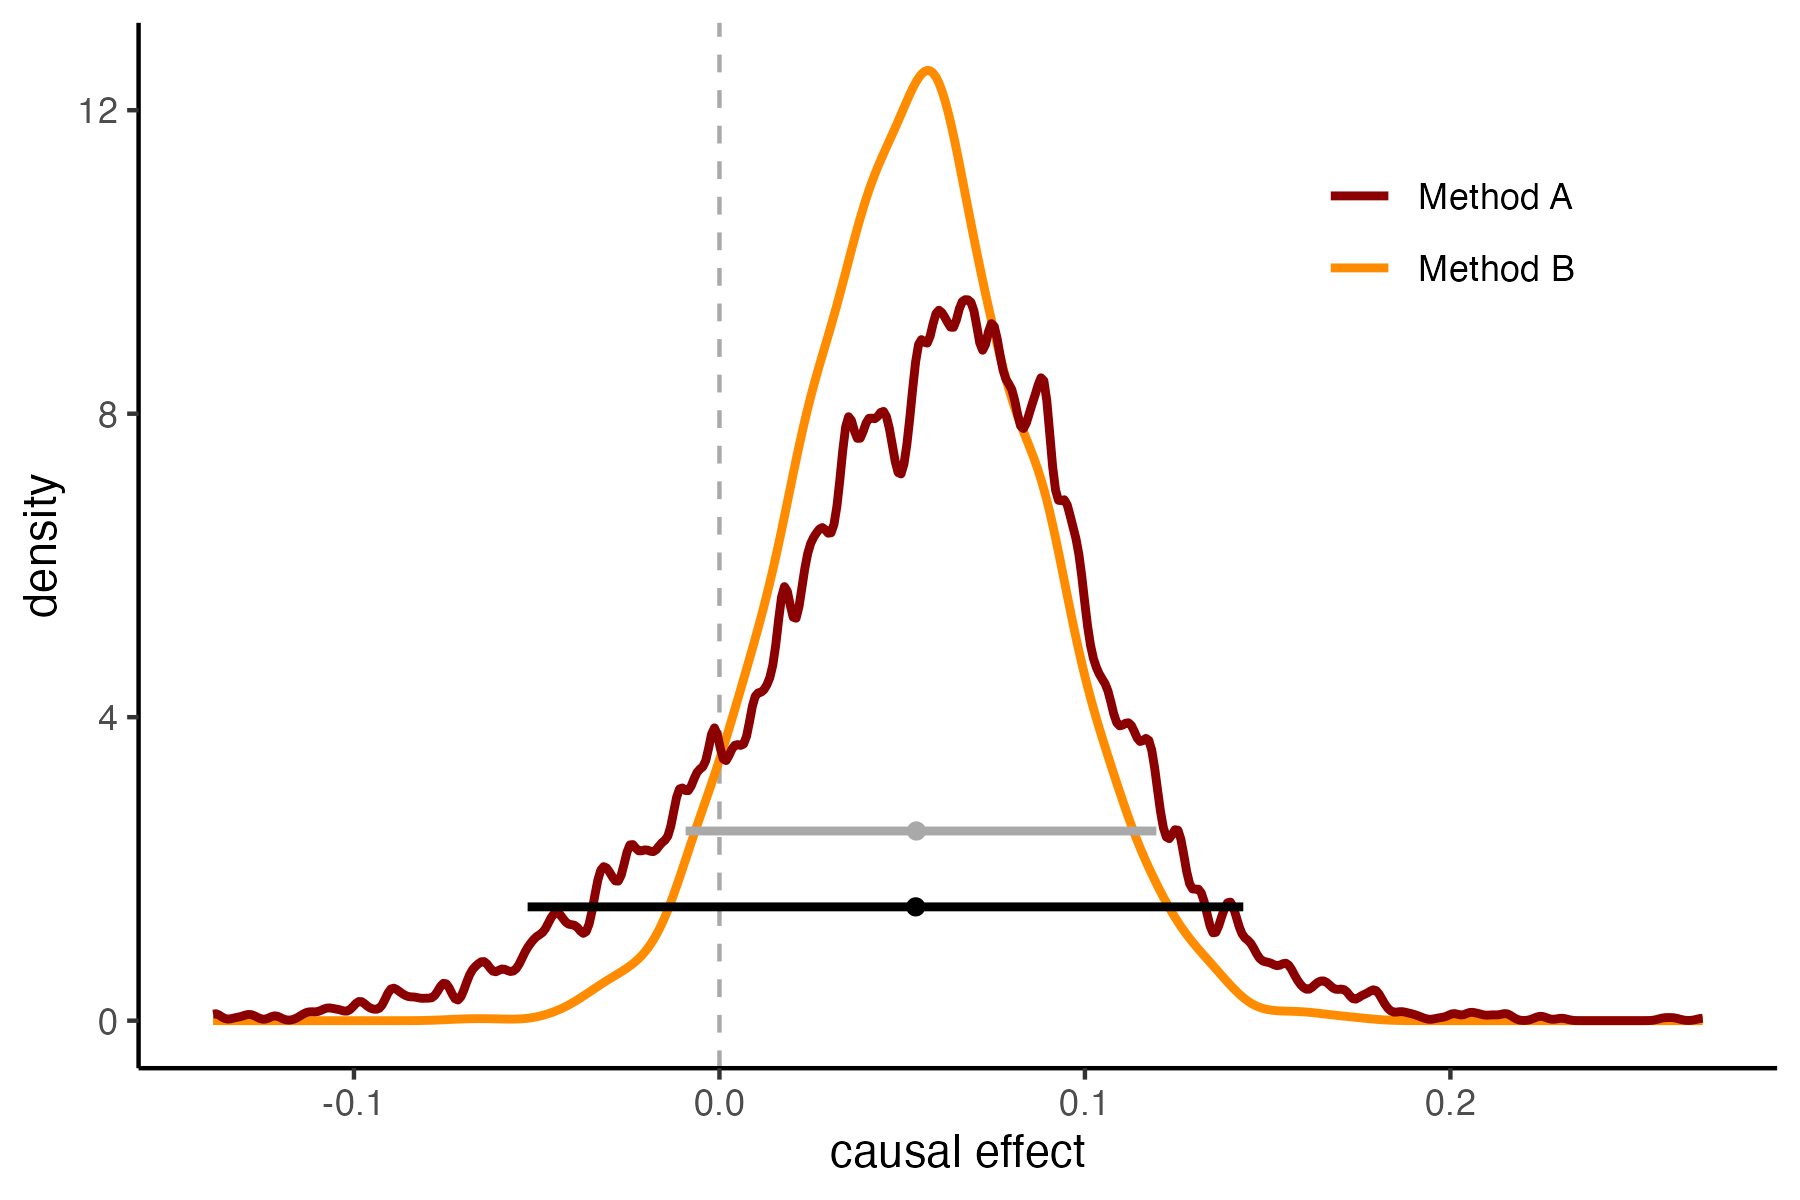
\includegraphics[width=0.8\linewidth]{img/gender_estimation_comparison.png}
    \caption{Causal effect estimation for \textsc{gender} as confound, using different estimation methods. Both methods yield the same mean, but the CI of \emph{Method B} (grey line) is narrower.}
    \label{fig:gender}
\end{figure}


\subsection{Experiment 2: Blood pressure as mediator}
In case 2 of Simpson’s paradox, blood pressure acts as a mediator between the drug and the patients’ recovery. 
We can estimate the chances of recovery simply as
$$P\left(R=1\mid \mathdo(D=d)\right)=P\left(R=1\mid D=d\right)$$
\textsc{blood pressure} is left out of this equation alltogether. 
\marginnote{In some cases, we don't want to compute the total causal effect, but only the direct causal effect, i.e. what effect does $D$ have on $R$ without the mediator $B$. In these cases, we would need to fit \textsc{recovery} to \textsc{drug intake} and \textsc{blood pressure}.}
After all, we’re only interested in the total causal effect of the drug, so to us it doesn't matter whether this effect takes place directly, or via changing the blood pressure.
Therefore, we fit \textsc{recovery} to \textsc{drug intake}.

\begin{minipage}[]{\textwidth}
\begin{lstlisting}[language=R]
# Estimate the distribution of recovery rates as predicted by drug intake
fit_recovery_bp <- brm(
  formula = recover ~ drug,
  data = data_SP_long,
  family = bernoulli(link = "logit"),
  iter = n_iter
)
\end{lstlisting}
\end{minipage}

\vspace{-0.5cm}
Because \textsc{drug intake} is the only predictive factor in our model, and the do-operation on \textsc{drug intake} has no effect (all causal links remain), we can obtain our posterior estimates of recovery rates with and without drug use by simply extracting the posterior draws that the model generated during fitting, and filter them according to the value of \textsc{drug intake}. 
\marginnote{In this instance, because $P(R=1\mid \mathdo(D=d))=P(R=1\mid D=d)$, there is no difference between observation and intervention}
We can do this with the \ri{filter\_cell\_draws} function from the \ri{faintr} package. 
\ri{filter\_cell\_draws} returns the posterior predictions of the linear predictor, therefore we need to apply the logistic function to obtain the expected values of the posterior predictive distribution. 

\begin{minipage}[]{\textwidth}
\begin{lstlisting}[language=R]
# posterior predictive samples for drug = 1 
posterior_DrugTaken_bp <-
  faintr::filter_cell_draws(fit_recovery_bp, drug == "Take") |>
  pull(draws) |>
  logistic()

# posterior predictive samples for drug = 0 
posterior_DrugRefused_bp <-
  faintr::filter_cell_draws(fit_recovery_bp, drug == "Refuse") |>
  pull(draws) |>
  logistic()

\end{lstlisting}
\end{minipage}

\vspace{-0.5cm}
With the posterior samples, we can continue as in case one: compute the means of both conditions to obtain the estimated chance of recovery with and without drug-taking, and then subtract the posterior samples of the \textsc{refuse} condition from the samples of the \textsc{take} condition to obtain the estimate of the causal effect of \textsc{drug intake} on \textsc{recovery}. 

\begin{minipage}[]{\textwidth}
\begin{rc}
> summarize_posterior(posterior_DrugRefused_bp, posterior_DrugTaken_bp)
# A tibble: 3 x 4
  condition     CI_lower    mean CI_upper
  <fct>            <dbl>   <dbl>    <dbl>
1 take drug        0.733  0.779    0.821 
2 refuse drug      0.783  0.825    0.863 
3 causal effect   -0.107 -0.0457   0.0127
\end{rc}
\end{minipage}

\vspace{-0.5cm}
We can see that taking the drug yields an estimated 78\% chance of recovery, while not taking it leads to a 83\% chance.
The causal effect is estimated to be -5\%, such that taking the drug is estimated to have detrimental effects on recovery.
As in the first experiment, the CI includes 0, such that we can't discard the null hypothesis.

\begin{figure}
    \centering
    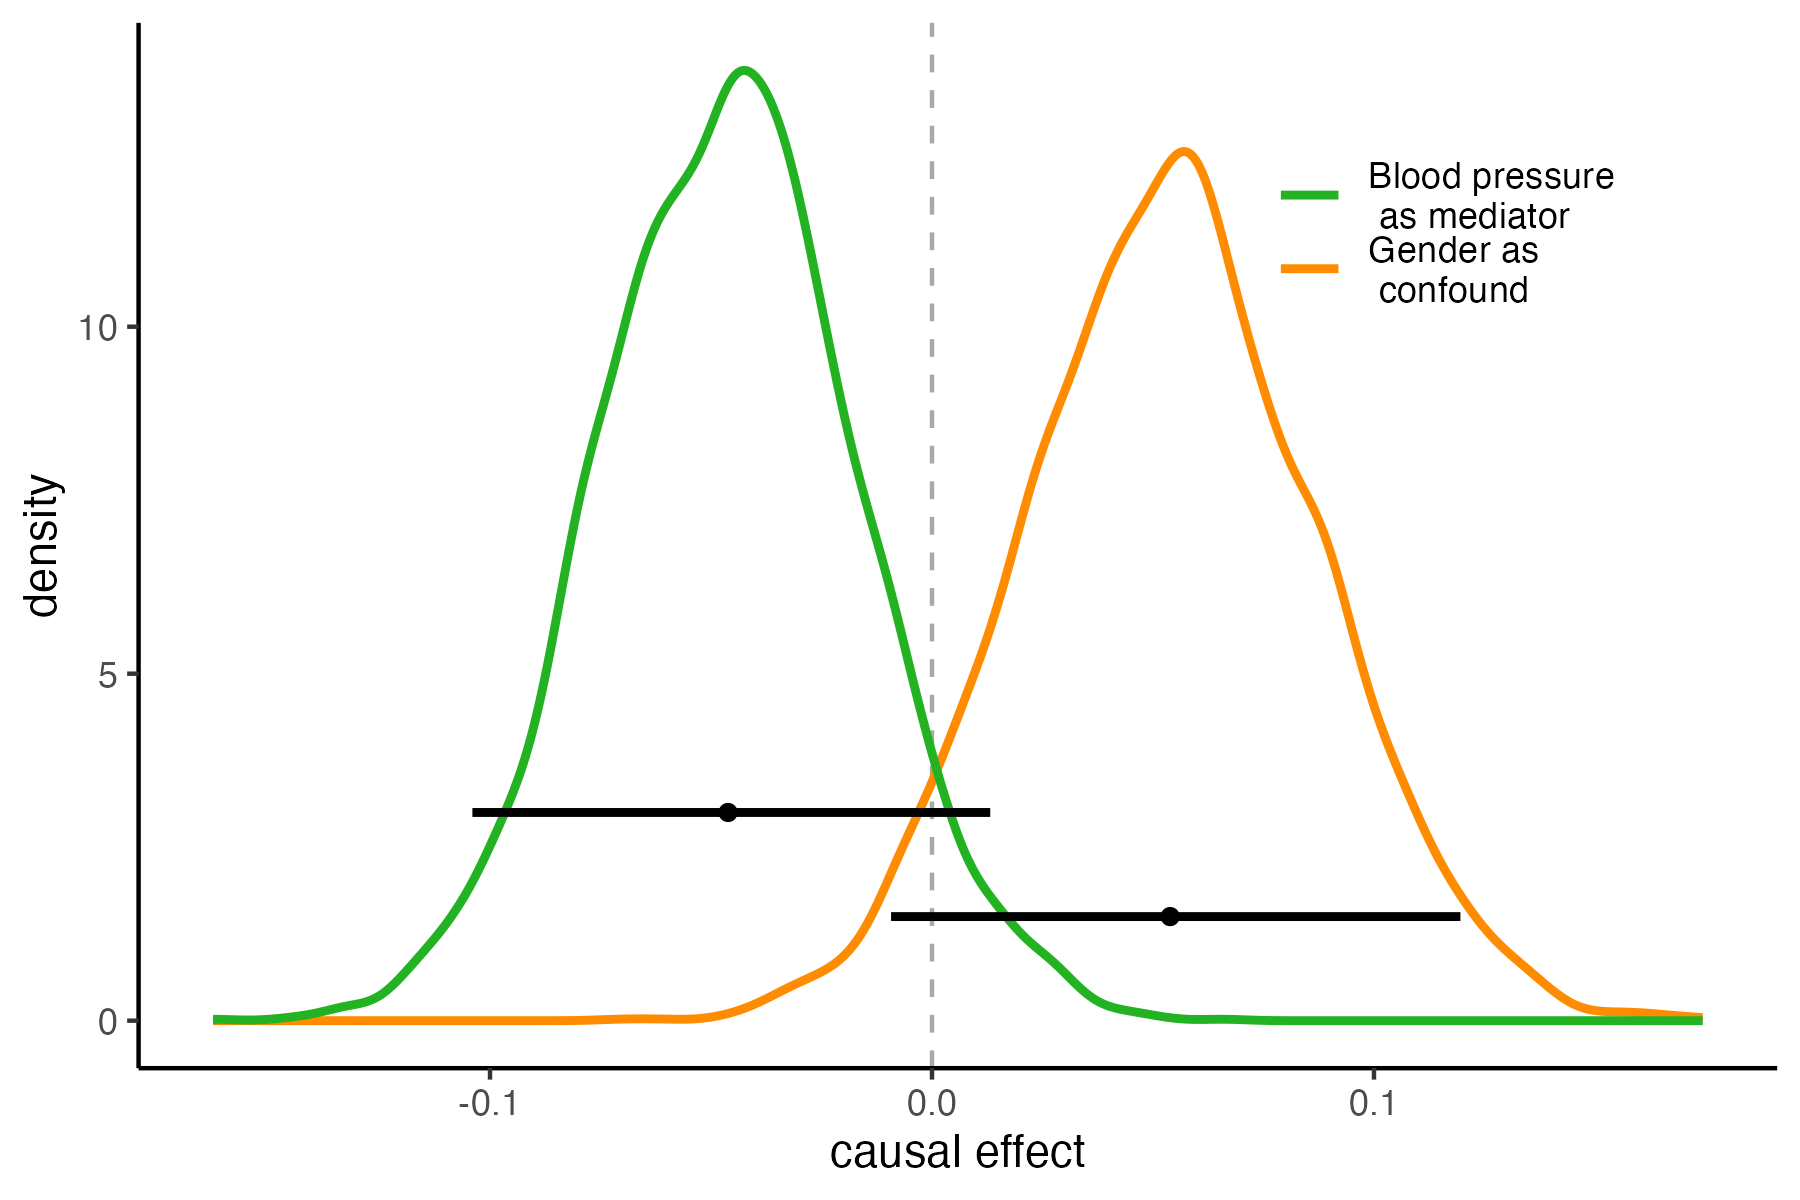
\includegraphics[width=0.8\linewidth]{img/posterior_causal_effect_smooth.png}
    \caption{Posterior distributions of the causal effect for both experiments. Bold Black lines indicate CIs, the means are shown as black dots.}
    \label{fig:posteriors}
\end{figure}

Taking a step back, what can we learn from these hypothetical experiments?
The data for both experiments was identical.
Despite that, the outcomes were different: even though both causal effects were not significant, they point to different directions, as can be seen in Figure \ref{fig:posteriors}.
This illustrates the importance of choosing the correct causal structure. 
Going beyond our hypothetical experiments, we showed that the \docalc can, in some scenarios, be used to estimate causal effects, even if the data at hand stems from observational studies.
To estimate the causal effects, both frequentist (MLE) and Bayesian methods yield similar results, however, only with the Bayesian approach do we get a measure of certainty for our results.

\printbibliography[heading=bibintoc]

\end{document}
